\documentclass[12pt,oneside]{book}

% PACCHETTI
\usepackage{tabto}              % strumento per inserire tab nel testo
\usepackage[                    % geometria della pagina
    a4paper,
    inner=2cm,
    outer=3cm,
    top=3cm,
    bottom=3cm,
    bindingoffset=1.2cm
]{geometry}
\usepackage[utf8]{inputenc}     % 3 pacchetti per l'italiano
\usepackage[italian]{babel}
\usepackage[T1]{fontenc}
\usepackage{titlesec}           % custom chapter titles

\usepackage{fancyhdr}
\usepackage[arrowdel]{physics} 

\usepackage{graphicx}           % IMMAGINI
\graphicspath{ {./images/} }


% INFORMAZIONI SUL DOCUMENTO
\title{\Large{\textbf{Fisica 1}}}
\author{Enrico Bragastini}
\titleformat{\chapter}[display]{\normalfont\bfseries}{}{0pt}{\LARGE}


% CONTENUTO
\begin{document}
\pagestyle{fancy}
\fancyhf{}
\rhead{}
\lhead{\nouppercase\leftmark}
\cfoot{\thepage}
\frontmatter

% Prima pagina - Titolo
\maketitle
\tableofcontents

\mainmatter
\chapter{Nozioni di base}
\section{Misura di una grandezza}
La misura di una grandezza può avvenire mediante un dispositivo misurabile
oppure in confronto con un'altra grandezza fisica omogenea di riferimento costante.

L'espressione di una grandezza fisica avviene nella forma: Numero + \underline{Unità di Misura}

\section{Grandezze fisiche fondamentali e derivate}
\subsection{Grandezze fisiche fondamentali}
Le grandezze fisiche fondamentali sono:
\begin{itemize}
    \item Lunghezza                 \tabto{8cm} [L]
    \item Massa                     \tabto{8cm}  [M]
    \item Tempo                     \tabto{8cm}  [t]
    \item Intensità Di Corrente     \tabto{8cm}  [i]
    \item Temperatura Assoluta      \tabto{8cm}  [T]
\end{itemize}

\subsection{Grandezze fisiche derivate}
Le grandezze fisiche derivate sono:
\begin{itemize}
    \item Superficie
    \item Volume
    \item Velocità
    \item Accelerazione
    \item Forza
    \item Pressione
    \item ...
\end{itemize}

\section{Sistemi di Unità di Misura}
\begin{center}
    \bgroup
    \def\arraystretch{1.5}
    \begin{tabular}{ |c| c c c c c|}
        \hline
        SISTEMA     & Lunghezza & Massa & Tempo & Corrente & Temperatura \\
        \hline
        MKS (s. i.) & m         & kg    & s     & A        & °K          \\
        \hline
        cgs         & cm        & g     & s     & A        & °K          \\
        \hline
    \end{tabular}
    \egroup
\end{center}

\subsection{Ulteriori Unità di Misura}
Esistono ulteriori sistemi di unità di misura che permettono di avere maggiore comodità
nelle misurazioni di particolari grandezze.
Se ne elencano alcuni:

\begin{enumerate}
    \item Lunghezza:    \tabto{3cm} Ångströms, Anno-Luce
    \item Tempo:        \tabto{3cm} Minuto, Ora
    \item Volume:       \tabto{3cm} Litro
    \item Velocità:     \tabto{3cm} Chilometro/Ora
    \item Pressione:    \tabto{3cm} Atmosfera, Millimetro di mercurio
    \item Energia:      \tabto{3cm} Elettrovolt, Chilovattora
\end{enumerate}

\section{Notazione Scientifica}
Per i numeri particolarmente grandi o piccoli risulta comodo rappresentarli
in \textbf{Notazione Scientifica} utilizzando le potenze del 10.

(Da integrare)

\section{Analisi Dimensionale}
L'analisi dimensionale è utile per controllare che una formula sia giusta o per dedurre come deve
essere una certa formula.
Le dimensioni possono essere trattate come quantità algebriche. Due membri della stessa equazione devono avere le
stesse dimensioni.

(Da integrare)

\section{Sistemi di Coordinate}
\subsection{Coordinate cartesiane}
\subsection{Coordinate scalari}

\section{Grandezze scalari e grandezze vettoriali}
\subsection{Grandezza scalare}
Una \textbf{grandezza scalare} è una grandezza specificata solamente da un valore numerico.

\subsection{Grandezza vettoriale}
Una \textbf{grandezza vettoriale} è una grandezza specificata da un valore numerico, detto \textbf{modulo}, e da una direzione orientata.

~\newline
Esempio di vettore:
\begin{equation*}
    \vec{A}
\end{equation*}

\subsubsection{Vettori uguali}
Due vettori $\vec{A}$ e $\vec{B}$ sono \textbf{uguali} se sono uguali i loro \emph{moduli}, la \emph{direzione} e il \emph{verso}.
L'uguaglianza è \emph{indipendente dall'origine}, ovvero i vettori possono essere traslati sul grafico in base alla necessità
senza che venga persa la loro uguaglianza.

\section{Operazioni tra vettori}
\subsection{Somma (metodo grafico)}
La somma tra vettori può essere svolta rapidamente in modo grafico mediante il metodo \textbf{punta-coda}.

In generale, se si vogliono sommare due spostamenti rappresentati dai due vettori a vettore e b vettore come di seguito rappresentato
\begin{figure}[h]
    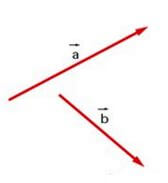
\includegraphics[scale=0.5]{vettori_da_sommare}
    \centering
\end{figure}

Spostiamo uno dei due vettori in modo tale che la sua coda coincida con la punta del primo vettore.

Riferendoci al nostro caso, spostiamo il vettore $\vec{b}$ vettore in modo tale che la sua coda coincida con la
punta del vettore $\vec{a}$, come di seguito rappresentato:
\begin{figure}[h]
    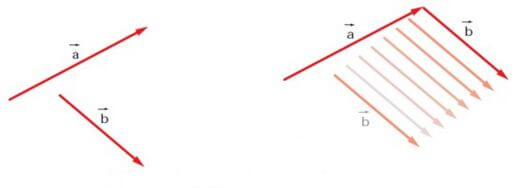
\includegraphics[scale=0.5]{punta_coda}
    \centering
\end{figure}

Come è possibile notare dalla figura precedente lo spostamento del vettore $\vec{b}$ deve essere effettuato in modo
tale che la freccia rimanga sempre parallela a se stessa.
Lo spostamento totale si ottiene unendo la coda del vettore $\vec{a}$ con la punta del vettore $\vec{a}$, come di seguito
rappresentato:
\begin{figure}[h]
    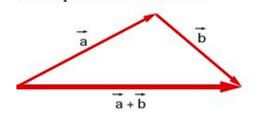
\includegraphics[scale=0.5]{vettori_sommati}
    \centering
\end{figure}

Si noti che in generale il modulo del vettore somma non è uguale alla somma dei moduli dei singoli spostamenti.

\subsection{Opposto di un vettore}
L'\textbf{opposto di un vettore} $\vec{A}$ è definito come il vettore che sommato a $\vec{A}$ permette di ottenere 0.
\begin{equation*}
    \vec{A} + (- \vec{A} ) = 0
\end{equation*}
Il vettore $(-\vec{A})$ è quindi un vettore che ha lo \textbf{stesso modulo} di $\vec{A}$, con la \textbf{stessa direzione} ma di \textbf{verso opposto}.

\subsection{Sottrazione tra vettori}
La \textbf{sottrazione tra vettori} si ottiene sfruttando la definizione di \emph{vettore opposto}.
Quindi, si vuole sottrarre il vettore $\vec{B}$ al vettore $\vec{A}$, basta \emph{sommarne l'opposto}.
\begin{equation*}
    \vec{A} - \vec{B} = \vec{A} + (- \vec{B})
\end{equation*}

\subsection{Prodotto tra un vettore e uno scalare}
\begin{itemize}
    \item Se un vettore $\vec{A}$ viene moltiplicato per una quantità scalare positiva $m$,
          allora il prodotto è $m\vec{A}$ e possiede la stessa direzione di A e modulo $mA$.
    \item Se un vettore $\vec{A}$ viene moltiplicato per una quantità scalare negativa $-m$,
          allora il prodotto è $-m\vec{A}$ e possiede direzione opposta di A e modulo $mA$.

\end{itemize}

\end{document}